% Options for packages loaded elsewhere
\PassOptionsToPackage{unicode}{hyperref}
\PassOptionsToPackage{hyphens}{url}
\PassOptionsToPackage{dvipsnames,svgnames,x11names}{xcolor}
%
\documentclass[
]{article}

\usepackage{amsmath,amssymb}
\usepackage{iftex}
\ifPDFTeX
  \usepackage[T1]{fontenc}
  \usepackage[utf8]{inputenc}
  \usepackage{textcomp} % provide euro and other symbols
\else % if luatex or xetex
  \usepackage{unicode-math}
  \defaultfontfeatures{Scale=MatchLowercase}
  \defaultfontfeatures[\rmfamily]{Ligatures=TeX,Scale=1}
\fi
\usepackage{lmodern}
\ifPDFTeX\else  
    % xetex/luatex font selection
\fi
% Use upquote if available, for straight quotes in verbatim environments
\IfFileExists{upquote.sty}{\usepackage{upquote}}{}
\IfFileExists{microtype.sty}{% use microtype if available
  \usepackage[]{microtype}
  \UseMicrotypeSet[protrusion]{basicmath} % disable protrusion for tt fonts
}{}
\makeatletter
\@ifundefined{KOMAClassName}{% if non-KOMA class
  \IfFileExists{parskip.sty}{%
    \usepackage{parskip}
  }{% else
    \setlength{\parindent}{0pt}
    \setlength{\parskip}{6pt plus 2pt minus 1pt}}
}{% if KOMA class
  \KOMAoptions{parskip=half}}
\makeatother
\usepackage{xcolor}
\setlength{\emergencystretch}{3em} % prevent overfull lines
\setcounter{secnumdepth}{-\maxdimen} % remove section numbering
% Make \paragraph and \subparagraph free-standing
\makeatletter
\ifx\paragraph\undefined\else
  \let\oldparagraph\paragraph
  \renewcommand{\paragraph}{
    \@ifstar
      \xxxParagraphStar
      \xxxParagraphNoStar
  }
  \newcommand{\xxxParagraphStar}[1]{\oldparagraph*{#1}\mbox{}}
  \newcommand{\xxxParagraphNoStar}[1]{\oldparagraph{#1}\mbox{}}
\fi
\ifx\subparagraph\undefined\else
  \let\oldsubparagraph\subparagraph
  \renewcommand{\subparagraph}{
    \@ifstar
      \xxxSubParagraphStar
      \xxxSubParagraphNoStar
  }
  \newcommand{\xxxSubParagraphStar}[1]{\oldsubparagraph*{#1}\mbox{}}
  \newcommand{\xxxSubParagraphNoStar}[1]{\oldsubparagraph{#1}\mbox{}}
\fi
\makeatother

\usepackage{color}
\usepackage{fancyvrb}
\newcommand{\VerbBar}{|}
\newcommand{\VERB}{\Verb[commandchars=\\\{\}]}
\DefineVerbatimEnvironment{Highlighting}{Verbatim}{commandchars=\\\{\}}
% Add ',fontsize=\small' for more characters per line
\usepackage{framed}
\definecolor{shadecolor}{RGB}{241,243,245}
\newenvironment{Shaded}{\begin{snugshade}}{\end{snugshade}}
\newcommand{\AlertTok}[1]{\textcolor[rgb]{0.68,0.00,0.00}{#1}}
\newcommand{\AnnotationTok}[1]{\textcolor[rgb]{0.37,0.37,0.37}{#1}}
\newcommand{\AttributeTok}[1]{\textcolor[rgb]{0.40,0.45,0.13}{#1}}
\newcommand{\BaseNTok}[1]{\textcolor[rgb]{0.68,0.00,0.00}{#1}}
\newcommand{\BuiltInTok}[1]{\textcolor[rgb]{0.00,0.23,0.31}{#1}}
\newcommand{\CharTok}[1]{\textcolor[rgb]{0.13,0.47,0.30}{#1}}
\newcommand{\CommentTok}[1]{\textcolor[rgb]{0.37,0.37,0.37}{#1}}
\newcommand{\CommentVarTok}[1]{\textcolor[rgb]{0.37,0.37,0.37}{\textit{#1}}}
\newcommand{\ConstantTok}[1]{\textcolor[rgb]{0.56,0.35,0.01}{#1}}
\newcommand{\ControlFlowTok}[1]{\textcolor[rgb]{0.00,0.23,0.31}{\textbf{#1}}}
\newcommand{\DataTypeTok}[1]{\textcolor[rgb]{0.68,0.00,0.00}{#1}}
\newcommand{\DecValTok}[1]{\textcolor[rgb]{0.68,0.00,0.00}{#1}}
\newcommand{\DocumentationTok}[1]{\textcolor[rgb]{0.37,0.37,0.37}{\textit{#1}}}
\newcommand{\ErrorTok}[1]{\textcolor[rgb]{0.68,0.00,0.00}{#1}}
\newcommand{\ExtensionTok}[1]{\textcolor[rgb]{0.00,0.23,0.31}{#1}}
\newcommand{\FloatTok}[1]{\textcolor[rgb]{0.68,0.00,0.00}{#1}}
\newcommand{\FunctionTok}[1]{\textcolor[rgb]{0.28,0.35,0.67}{#1}}
\newcommand{\ImportTok}[1]{\textcolor[rgb]{0.00,0.46,0.62}{#1}}
\newcommand{\InformationTok}[1]{\textcolor[rgb]{0.37,0.37,0.37}{#1}}
\newcommand{\KeywordTok}[1]{\textcolor[rgb]{0.00,0.23,0.31}{\textbf{#1}}}
\newcommand{\NormalTok}[1]{\textcolor[rgb]{0.00,0.23,0.31}{#1}}
\newcommand{\OperatorTok}[1]{\textcolor[rgb]{0.37,0.37,0.37}{#1}}
\newcommand{\OtherTok}[1]{\textcolor[rgb]{0.00,0.23,0.31}{#1}}
\newcommand{\PreprocessorTok}[1]{\textcolor[rgb]{0.68,0.00,0.00}{#1}}
\newcommand{\RegionMarkerTok}[1]{\textcolor[rgb]{0.00,0.23,0.31}{#1}}
\newcommand{\SpecialCharTok}[1]{\textcolor[rgb]{0.37,0.37,0.37}{#1}}
\newcommand{\SpecialStringTok}[1]{\textcolor[rgb]{0.13,0.47,0.30}{#1}}
\newcommand{\StringTok}[1]{\textcolor[rgb]{0.13,0.47,0.30}{#1}}
\newcommand{\VariableTok}[1]{\textcolor[rgb]{0.07,0.07,0.07}{#1}}
\newcommand{\VerbatimStringTok}[1]{\textcolor[rgb]{0.13,0.47,0.30}{#1}}
\newcommand{\WarningTok}[1]{\textcolor[rgb]{0.37,0.37,0.37}{\textit{#1}}}

\providecommand{\tightlist}{%
  \setlength{\itemsep}{0pt}\setlength{\parskip}{0pt}}\usepackage{longtable,booktabs,array}
\usepackage{calc} % for calculating minipage widths
% Correct order of tables after \paragraph or \subparagraph
\usepackage{etoolbox}
\makeatletter
\patchcmd\longtable{\par}{\if@noskipsec\mbox{}\fi\par}{}{}
\makeatother
% Allow footnotes in longtable head/foot
\IfFileExists{footnotehyper.sty}{\usepackage{footnotehyper}}{\usepackage{footnote}}
\makesavenoteenv{longtable}
\usepackage{graphicx}
\makeatletter
\def\maxwidth{\ifdim\Gin@nat@width>\linewidth\linewidth\else\Gin@nat@width\fi}
\def\maxheight{\ifdim\Gin@nat@height>\textheight\textheight\else\Gin@nat@height\fi}
\makeatother
% Scale images if necessary, so that they will not overflow the page
% margins by default, and it is still possible to overwrite the defaults
% using explicit options in \includegraphics[width, height, ...]{}
\setkeys{Gin}{width=\maxwidth,height=\maxheight,keepaspectratio}
% Set default figure placement to htbp
\makeatletter
\def\fps@figure{htbp}
\makeatother

\usepackage{fvextra}
\DefineVerbatimEnvironment{Highlighting}{Verbatim}{breaklines,commandchars=\\\{\}}
\makeatletter
\@ifpackageloaded{caption}{}{\usepackage{caption}}
\AtBeginDocument{%
\ifdefined\contentsname
  \renewcommand*\contentsname{Table of contents}
\else
  \newcommand\contentsname{Table of contents}
\fi
\ifdefined\listfigurename
  \renewcommand*\listfigurename{List of Figures}
\else
  \newcommand\listfigurename{List of Figures}
\fi
\ifdefined\listtablename
  \renewcommand*\listtablename{List of Tables}
\else
  \newcommand\listtablename{List of Tables}
\fi
\ifdefined\figurename
  \renewcommand*\figurename{Figure}
\else
  \newcommand\figurename{Figure}
\fi
\ifdefined\tablename
  \renewcommand*\tablename{Table}
\else
  \newcommand\tablename{Table}
\fi
}
\@ifpackageloaded{float}{}{\usepackage{float}}
\floatstyle{ruled}
\@ifundefined{c@chapter}{\newfloat{codelisting}{h}{lop}}{\newfloat{codelisting}{h}{lop}[chapter]}
\floatname{codelisting}{Listing}
\newcommand*\listoflistings{\listof{codelisting}{List of Listings}}
\makeatother
\makeatletter
\makeatother
\makeatletter
\@ifpackageloaded{caption}{}{\usepackage{caption}}
\@ifpackageloaded{subcaption}{}{\usepackage{subcaption}}
\makeatother

\ifLuaTeX
  \usepackage{selnolig}  % disable illegal ligatures
\fi
\usepackage{bookmark}

\IfFileExists{xurl.sty}{\usepackage{xurl}}{} % add URL line breaks if available
\urlstyle{same} % disable monospaced font for URLs
\hypersetup{
  pdftitle={30538 Problem Set 2: Parking Tickets},
  pdfauthor={Emma Brady},
  colorlinks=true,
  linkcolor={blue},
  filecolor={Maroon},
  citecolor={Blue},
  urlcolor={Blue},
  pdfcreator={LaTeX via pandoc}}


\title{30538 Problem Set 2: Parking Tickets}
\author{Emma Brady}
\date{2024-10-19}

\begin{document}
\maketitle


\begin{enumerate}
\def\labelenumi{\arabic{enumi}.}
\tightlist
\item
  ``This submission is my work alone and complies with the 30538
  integrity policy.'' Add your initials to indicate your agreement:
  **\E\B**
\item
  ``I have uploaded the names of anyone I worked with on the problem set
  \textbf{\href{https://docs.google.com/forms/d/1-zzHx762odGlpVWtgdIC55vqF-j3gqdAp6Pno1rIGK0/edit}{here}}''
  **\_\_** (1 point)
\item
  Late coins used this pset: **\_\_\emph{* Late coins left after
  submission: **\_\_}*
\item
  Knit your \texttt{ps2.qmd} to make \texttt{ps2.pdf}.

  \begin{itemize}
  \tightlist
  \item
    The PDF should not be more than 25 pages. Use \texttt{head()} and
    re-size figures when appropriate.
  \end{itemize}
\item
  Push \texttt{ps2.qmd} and \texttt{ps2.pdf} to your github repo. It is
  fine to use Github Desktop.
\item
  Submit \texttt{ps2.pdf} via Gradescope (4 points)
\item
  Tag your submission in Gradescope
\end{enumerate}

\begin{Shaded}
\begin{Highlighting}[]
\ImportTok{import}\NormalTok{ pandas }\ImportTok{as}\NormalTok{ pd}
\ImportTok{import}\NormalTok{ altair }\ImportTok{as}\NormalTok{ alt}
\NormalTok{alt.renderers.enable(}\StringTok{"png"}\NormalTok{)}
\ImportTok{import}\NormalTok{ time}

\ImportTok{import}\NormalTok{ warnings }
\NormalTok{warnings.filterwarnings(}\StringTok{\textquotesingle{}ignore\textquotesingle{}}\NormalTok{)}
\end{Highlighting}
\end{Shaded}

\subsection{Data cleaning continued (15
points)}\label{data-cleaning-continued-15-points}

\begin{enumerate}
\def\labelenumi{\arabic{enumi}.}
\tightlist
\item
  Read csv file
\end{enumerate}

\begin{Shaded}
\begin{Highlighting}[]
\NormalTok{df }\OperatorTok{=}\NormalTok{ pd.read\_csv(}\StringTok{\textquotesingle{}data/parking\_tickets\_one\_percent.csv\textquotesingle{}}\NormalTok{)}
\end{Highlighting}
\end{Shaded}

Function that creates a new data frame with variables and NA Count

\begin{Shaded}
\begin{Highlighting}[]
\KeywordTok{def}\NormalTok{ na\_function(df):}
    \CommentTok{"""create a data frame with variables and NA count"""}
\NormalTok{    count\_na }\OperatorTok{=}\NormalTok{ pd.DataFrame(\{}
        \StringTok{\textquotesingle{}Variable\textquotesingle{}}\NormalTok{: df.columns,}
        \StringTok{\textquotesingle{}NA\textquotesingle{}}\NormalTok{: df.isna().}\BuiltInTok{sum}\NormalTok{()}
\NormalTok{    \})}
    \ControlFlowTok{return}\NormalTok{ count\_na}
\end{Highlighting}
\end{Shaded}

Testing out the function

\begin{Shaded}
\begin{Highlighting}[]
\CommentTok{\#\#Creating test dataframe}
\NormalTok{test\_df }\OperatorTok{=}\NormalTok{ pd.DataFrame(\{}
    \StringTok{\textquotesingle{}test1\textquotesingle{}}\NormalTok{: [}\VariableTok{None}\NormalTok{, }\DecValTok{1}\NormalTok{, }\DecValTok{1}\NormalTok{, }\DecValTok{1}\NormalTok{, }\DecValTok{1}\NormalTok{],}
    \StringTok{\textquotesingle{}test2\textquotesingle{}}\NormalTok{: [}\DecValTok{2}\NormalTok{, }\VariableTok{None}\NormalTok{, }\DecValTok{2}\NormalTok{, }\VariableTok{None}\NormalTok{, }\DecValTok{2}\NormalTok{],}
    \StringTok{\textquotesingle{}test3\textquotesingle{}}\NormalTok{: [}\DecValTok{3}\NormalTok{, }\DecValTok{3}\NormalTok{, }\VariableTok{None}\NormalTok{, }\VariableTok{None}\NormalTok{, }\VariableTok{None}\NormalTok{],}
    \StringTok{\textquotesingle{}test4\textquotesingle{}}\NormalTok{: [}\DecValTok{4}\NormalTok{, }\DecValTok{4}\NormalTok{, }\DecValTok{4}\NormalTok{, }\DecValTok{4}\NormalTok{, }\DecValTok{4}\NormalTok{]}
\NormalTok{\})}

\CommentTok{\#\#testing the function on the test dataframe}

\NormalTok{testing\_na }\OperatorTok{=}\NormalTok{ na\_function(test\_df)}
\BuiltInTok{print}\NormalTok{(testing\_na)}
\end{Highlighting}
\end{Shaded}

\begin{verbatim}
      Variable  NA
test1    test1   1
test2    test2   2
test3    test3   3
test4    test4   0
\end{verbatim}

Use the function on the parking tickets data frame

\begin{Shaded}
\begin{Highlighting}[]
\NormalTok{parking\_tickets\_na }\OperatorTok{=}\NormalTok{ na\_function(df)}
\BuiltInTok{print}\NormalTok{(parking\_tickets\_na)}
\end{Highlighting}
\end{Shaded}

\begin{verbatim}
                                    Variable      NA
Unnamed: 0                        Unnamed: 0       0
ticket_number                  ticket_number       0
issue_date                        issue_date       0
violation_location        violation_location       0
license_plate_number    license_plate_number       0
license_plate_state      license_plate_state      97
license_plate_type        license_plate_type    2054
zipcode                              zipcode   54115
violation_code                violation_code       0
violation_description  violation_description       0
unit                                    unit      29
unit_description            unit_description       0
vehicle_make                    vehicle_make       0
fine_level1_amount        fine_level1_amount       0
fine_level2_amount        fine_level2_amount       0
current_amount_due        current_amount_due       0
total_payments                total_payments       0
ticket_queue                    ticket_queue       0
ticket_queue_date          ticket_queue_date       0
notice_level                    notice_level   84068
hearing_disposition      hearing_disposition  259899
notice_number                  notice_number       0
officer                              officer       0
address                              address       0
\end{verbatim}

Referred to the following webpages:
https://saturncloud.io/blog/how-to-count-nan-values-in-a-pandas-dataframe-column/
https://www.geeksforgeeks.org/different-ways-to-create-pandas-dataframe/
https://stackoverflow.com/questions/45579525/returning-a-dataframe-in-python-function

\begin{enumerate}
\def\labelenumi{\arabic{enumi}.}
\setcounter{enumi}{1}
\tightlist
\item
  notice\_level, hearing\_disposition, and zipcode are missing more
  often than others.
\end{enumerate}

Notice level is missing often because if the field is blank no notice
was sent. All the NAs indicate that no notice was sent.

While hearing disposition is not defined in the data dictionary, it may
refer to whether there was a hearing disposition for the ticket, and the
NAs may indicate that there wasn't.

Zipcode refers to the ZIPcode associated with the vehicle registration,
and if the ticket is associated to a lack of vehicle registration than
there will be an NA there.

\begin{enumerate}
\def\labelenumi{\arabic{enumi}.}
\setcounter{enumi}{2}
\tightlist
\item
\end{enumerate}

\begin{Shaded}
\begin{Highlighting}[]
\CommentTok{\#\#Create a function that gives the corresponding value in the \textquotesingle{}violation\_code\textquotesingle{} column for any value in the \textquotesingle{}violation\_description\textquotesingle{} that contains the words "city sticker"}
\KeywordTok{def}\NormalTok{ city\_sticker\_function(df):}
\NormalTok{    sticker\_violation }\OperatorTok{=}\NormalTok{ df[df[}\StringTok{\textquotesingle{}violation\_description\textquotesingle{}}\NormalTok{].}\BuiltInTok{str}\NormalTok{.contains(}\StringTok{\textquotesingle{}NO CITY STICKER\textquotesingle{}}\NormalTok{)]}
    \ControlFlowTok{return}\NormalTok{ sticker\_violation[}\StringTok{\textquotesingle{}violation\_code\textquotesingle{}}\NormalTok{]}

\NormalTok{city\_sticker\_violation\_codes }\OperatorTok{=}\NormalTok{ city\_sticker\_function(df).unique()}
\BuiltInTok{print}\NormalTok{(city\_sticker\_violation\_codes)}
\end{Highlighting}
\end{Shaded}

\begin{verbatim}
['0964125' '0976170' '0964125B' '0964125C']
\end{verbatim}

\begin{Shaded}
\begin{Highlighting}[]
\CommentTok{\#\#check that each code pulled is for no city sticker}
\BuiltInTok{print}\NormalTok{(df[}\StringTok{\textquotesingle{}violation\_description\textquotesingle{}}\NormalTok{].loc[df[}\StringTok{\textquotesingle{}violation\_code\textquotesingle{}}\NormalTok{] }\OperatorTok{==} \StringTok{\textquotesingle{}0964125\textquotesingle{}}\NormalTok{].unique())}
\BuiltInTok{print}\NormalTok{(df[}\StringTok{\textquotesingle{}violation\_description\textquotesingle{}}\NormalTok{].loc[df[}\StringTok{\textquotesingle{}violation\_code\textquotesingle{}}\NormalTok{] }\OperatorTok{==} \StringTok{\textquotesingle{}0976170\textquotesingle{}}\NormalTok{].unique())}
\BuiltInTok{print}\NormalTok{(df[}\StringTok{\textquotesingle{}violation\_description\textquotesingle{}}\NormalTok{].loc[df[}\StringTok{\textquotesingle{}violation\_code\textquotesingle{}}\NormalTok{] }\OperatorTok{==} \StringTok{\textquotesingle{}0964125B\textquotesingle{}}\NormalTok{].unique())}
\BuiltInTok{print}\NormalTok{(df[}\StringTok{\textquotesingle{}violation\_description\textquotesingle{}}\NormalTok{].loc[df[}\StringTok{\textquotesingle{}violation\_code\textquotesingle{}}\NormalTok{] }\OperatorTok{==} \StringTok{\textquotesingle{}0964125C\textquotesingle{}}\NormalTok{].unique())}
\end{Highlighting}
\end{Shaded}

\begin{verbatim}
['NO CITY STICKER OR IMPROPER DISPLAY']
['NO CITY STICKER OR IMPROPER DISPLAY']
['NO CITY STICKER VEHICLE UNDER/EQUAL TO 16,000 LBS.']
['NO CITY STICKER VEHICLE OVER 16,000 LBS.']
\end{verbatim}

The original violation code was 0964125 and the new violation code is
0976170. Violation codes also included 0964125B for no city sticker on
vehicles under/equal to 16,000 lbs and 0964125C for no city sticker on
vehicles over 16,000 lbs.

\begin{enumerate}
\def\labelenumi{\arabic{enumi}.}
\setcounter{enumi}{3}
\tightlist
\item
\end{enumerate}

\begin{Shaded}
\begin{Highlighting}[]
\BuiltInTok{print}\NormalTok{(df[}\StringTok{\textquotesingle{}fine\_level1\_amount\textquotesingle{}}\NormalTok{].loc[df[}\StringTok{\textquotesingle{}violation\_code\textquotesingle{}}\NormalTok{] }\OperatorTok{==} \StringTok{\textquotesingle{}0964125\textquotesingle{}}\NormalTok{].unique())}
\end{Highlighting}
\end{Shaded}

\begin{verbatim}
[120]
\end{verbatim}

The cost of an initial offense for violation code 0964125 is \$120

\begin{Shaded}
\begin{Highlighting}[]
\BuiltInTok{print}\NormalTok{(df[}\StringTok{\textquotesingle{}fine\_level1\_amount\textquotesingle{}}\NormalTok{].loc[df[}\StringTok{\textquotesingle{}violation\_code\textquotesingle{}}\NormalTok{] }\OperatorTok{==} \StringTok{\textquotesingle{}0976170\textquotesingle{}}\NormalTok{].unique())}
\end{Highlighting}
\end{Shaded}

\begin{verbatim}
[120]
\end{verbatim}

The cost of an initial offense for violation code 0976170 is \$120

\begin{Shaded}
\begin{Highlighting}[]
\BuiltInTok{print}\NormalTok{(df[}\StringTok{\textquotesingle{}fine\_level1\_amount\textquotesingle{}}\NormalTok{].loc[df[}\StringTok{\textquotesingle{}violation\_code\textquotesingle{}}\NormalTok{] }\OperatorTok{==} \StringTok{\textquotesingle{}0964125B\textquotesingle{}}\NormalTok{].unique())}
\end{Highlighting}
\end{Shaded}

\begin{verbatim}
[200]
\end{verbatim}

The cost of an initial offense for violation code 0964125B is \$200.

\subsection{Revenue increase from ``missing city sticker'' tickets (20
Points)}\label{revenue-increase-from-missing-city-sticker-tickets-20-points}

\begin{enumerate}
\def\labelenumi{\arabic{enumi}.}
\tightlist
\item
  Create a new value for violation codes which combines the two city
  sticker violation codes.
\end{enumerate}

\begin{Shaded}
\begin{Highlighting}[]
\NormalTok{df[}\StringTok{\textquotesingle{}violation\_code\textquotesingle{}}\NormalTok{] }\OperatorTok{=}\NormalTok{ df[}\StringTok{\textquotesingle{}violation\_code\textquotesingle{}}\NormalTok{].replace([}\StringTok{\textquotesingle{}0964125\textquotesingle{}}\NormalTok{, }\StringTok{\textquotesingle{}0976170\textquotesingle{}}\NormalTok{, }\StringTok{\textquotesingle{}0964125B\textquotesingle{}}\NormalTok{], }\StringTok{\textquotesingle{}1111111\textquotesingle{}}\NormalTok{)}
\end{Highlighting}
\end{Shaded}

Collapse the data to capture the number of missing city sticker tickets
by month.

\begin{Shaded}
\begin{Highlighting}[]
\NormalTok{df[}\StringTok{\textquotesingle{}issue\_date\textquotesingle{}}\NormalTok{] }\OperatorTok{=}\NormalTok{ pd.to\_datetime(df[}\StringTok{\textquotesingle{}issue\_date\textquotesingle{}}\NormalTok{])}
\NormalTok{filtered\_df }\OperatorTok{=}\NormalTok{ df[df[}\StringTok{\textquotesingle{}violation\_code\textquotesingle{}}\NormalTok{] }\OperatorTok{==} \StringTok{\textquotesingle{}1111111\textquotesingle{}}\NormalTok{]}

\NormalTok{filtered\_df[}\StringTok{\textquotesingle{}month\textquotesingle{}}\NormalTok{] }\OperatorTok{=}\NormalTok{ filtered\_df[}\StringTok{\textquotesingle{}issue\_date\textquotesingle{}}\NormalTok{].dt.to\_period(}\StringTok{\textquotesingle{}M\textquotesingle{}}\NormalTok{)}
\NormalTok{stickers\_by\_month }\OperatorTok{=}\NormalTok{ filtered\_df.groupby(}\StringTok{\textquotesingle{}month\textquotesingle{}}\NormalTok{)[}\StringTok{\textquotesingle{}violation\_code\textquotesingle{}}\NormalTok{].count().reset\_index()}
\NormalTok{stickers\_by\_month[}\StringTok{\textquotesingle{}month\textquotesingle{}}\NormalTok{] }\OperatorTok{=}\NormalTok{ stickers\_by\_month[}\StringTok{\textquotesingle{}month\textquotesingle{}}\NormalTok{].astype(}\BuiltInTok{str}\NormalTok{)}
\end{Highlighting}
\end{Shaded}

Use Altair to plot the number of tickets over time

\begin{Shaded}
\begin{Highlighting}[]
\NormalTok{sticker\_violations\_by\_month\_chart }\OperatorTok{=}\NormalTok{ alt.Chart(stickers\_by\_month).mark\_line().encode(}
\NormalTok{    alt.X(}\StringTok{\textquotesingle{}month:O\textquotesingle{}}\NormalTok{, title}\OperatorTok{=}\StringTok{\textquotesingle{}Issue Month\textquotesingle{}}\NormalTok{),}
\NormalTok{    alt.Y(}\StringTok{\textquotesingle{}violation\_code:Q\textquotesingle{}}\NormalTok{, title}\OperatorTok{=}\StringTok{\textquotesingle{}City Sticker Violations\textquotesingle{}}\NormalTok{)}
\NormalTok{)}
\NormalTok{sticker\_violations\_by\_month\_chart}
\end{Highlighting}
\end{Shaded}

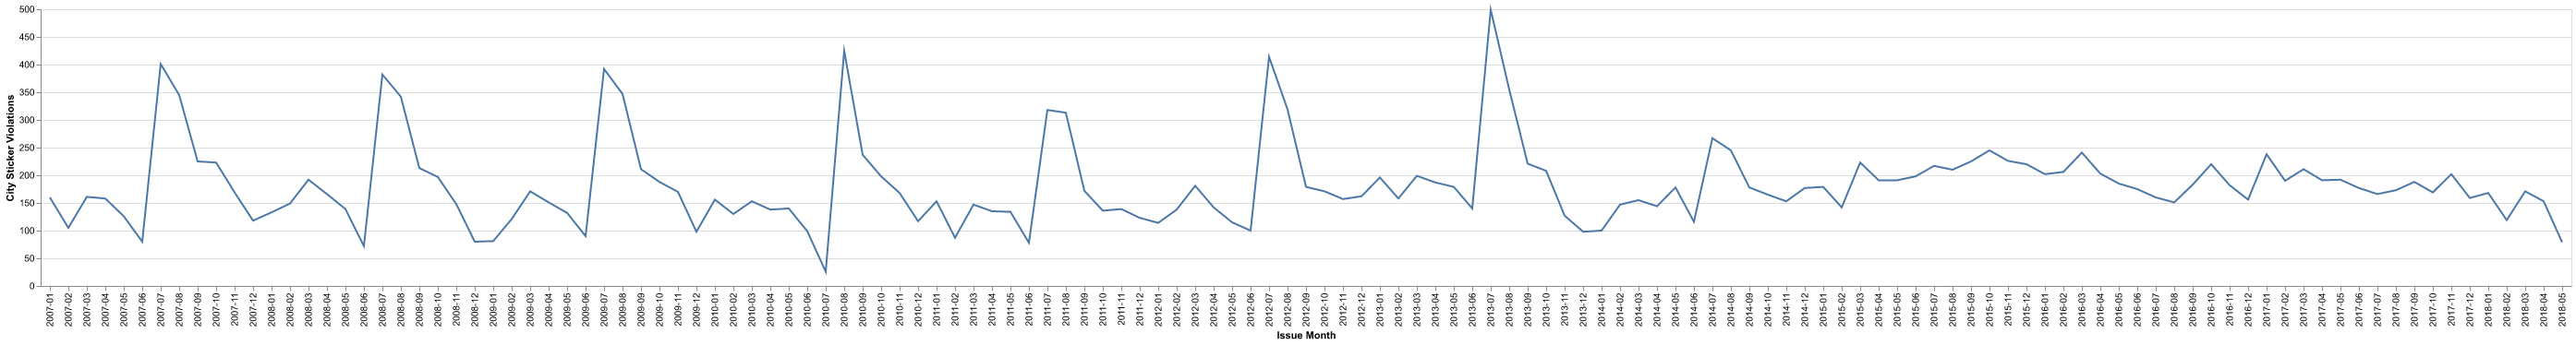
\includegraphics[width=29.05208in,height=3.89583in]{pset2_template_files/figure-pdf/cell-14-output-1.png}

Referred to the following page:
https://www.statology.org/pandas-group-by-month/

\begin{enumerate}
\def\labelenumi{\arabic{enumi}.}
\setcounter{enumi}{1}
\tightlist
\item
\item
\end{enumerate}

\begin{Shaded}
\begin{Highlighting}[]
\NormalTok{violations\_2011 }\OperatorTok{=}\NormalTok{ df[(df[}\StringTok{\textquotesingle{}violation\_code\textquotesingle{}}\NormalTok{] }\OperatorTok{==} \StringTok{\textquotesingle{}1111111\textquotesingle{}}\NormalTok{) }\OperatorTok{\&}\NormalTok{ (df[}\StringTok{\textquotesingle{}issue\_date\textquotesingle{}}\NormalTok{].dt.year }\OperatorTok{==} \DecValTok{2011}\NormalTok{)]}
\NormalTok{violations\_2011.shape[}\DecValTok{0}\NormalTok{]}
\end{Highlighting}
\end{Shaded}

\begin{verbatim}
1935
\end{verbatim}

In this 1\% sample of the data, there were 1935 sticker violation
tickets in 2011, implying that there were roughly 193,500 total sticker
violations. With an \$80 increase in the ticket charge, the city would
raise revenue by \$15,480,000.

\begin{enumerate}
\def\labelenumi{\arabic{enumi}.}
\setcounter{enumi}{3}
\tightlist
\item
\end{enumerate}

\begin{Shaded}
\begin{Highlighting}[]
\CommentTok{\#calculate total number of no city sticker violations in 2011}
\NormalTok{violations\_2011 }\OperatorTok{=}\NormalTok{ df[(df[}\StringTok{\textquotesingle{}violation\_code\textquotesingle{}}\NormalTok{] }\OperatorTok{==} \StringTok{\textquotesingle{}1111111\textquotesingle{}}\NormalTok{) }\OperatorTok{\&}\NormalTok{ (df[}\StringTok{\textquotesingle{}issue\_date\textquotesingle{}}\NormalTok{].dt.year }\OperatorTok{==} \DecValTok{2011}\NormalTok{)]}
\NormalTok{violations\_2011.shape[}\DecValTok{0}\NormalTok{]}
\end{Highlighting}
\end{Shaded}

\begin{verbatim}
1935
\end{verbatim}

\begin{Shaded}
\begin{Highlighting}[]
\CommentTok{\#calculate paid number of no city sticker violations in 2011}
\NormalTok{violations\_2011\_unpaid }\OperatorTok{=}\NormalTok{ df[(df[}\StringTok{\textquotesingle{}violation\_code\textquotesingle{}}\NormalTok{] }\OperatorTok{==} \StringTok{\textquotesingle{}1111111\textquotesingle{}}\NormalTok{) }\OperatorTok{\&}\NormalTok{ (df[}\StringTok{\textquotesingle{}issue\_date\textquotesingle{}}\NormalTok{].dt.year }\OperatorTok{==} \DecValTok{2011}\NormalTok{) }\OperatorTok{\&}\NormalTok{ (df[}\StringTok{\textquotesingle{}ticket\_queue\textquotesingle{}}\NormalTok{] }\OperatorTok{==} \StringTok{\textquotesingle{}Paid\textquotesingle{}}\NormalTok{)]}
\NormalTok{violations\_2011\_unpaid.shape[}\DecValTok{0}\NormalTok{]}
\end{Highlighting}
\end{Shaded}

\begin{verbatim}
1044
\end{verbatim}

There were 1935 no sticker violation tickets issued in this sample set
in 2011 and 1044 were paid, so there waas a repayment rate of 54\%.

\begin{Shaded}
\begin{Highlighting}[]
\CommentTok{\#calculate total number of no city sticker violations in 2012}
\NormalTok{violations\_2012 }\OperatorTok{=}\NormalTok{ df[(df[}\StringTok{\textquotesingle{}violation\_code\textquotesingle{}}\NormalTok{] }\OperatorTok{==} \StringTok{\textquotesingle{}1111111\textquotesingle{}}\NormalTok{) }\OperatorTok{\&}\NormalTok{ (df[}\StringTok{\textquotesingle{}issue\_date\textquotesingle{}}\NormalTok{].dt.year }\OperatorTok{==} \DecValTok{2012}\NormalTok{)]}
\NormalTok{violations\_2012.shape[}\DecValTok{0}\NormalTok{]}
\end{Highlighting}
\end{Shaded}

\begin{verbatim}
2192
\end{verbatim}

\begin{Shaded}
\begin{Highlighting}[]
\CommentTok{\#calculate paid number of no city sticker violations in 2012}
\NormalTok{violations\_2012\_unpaid }\OperatorTok{=}\NormalTok{ df[(df[}\StringTok{\textquotesingle{}violation\_code\textquotesingle{}}\NormalTok{] }\OperatorTok{==} \StringTok{\textquotesingle{}1111111\textquotesingle{}}\NormalTok{) }\OperatorTok{\&}\NormalTok{ (df[}\StringTok{\textquotesingle{}issue\_date\textquotesingle{}}\NormalTok{].dt.year }\OperatorTok{==} \DecValTok{2012}\NormalTok{) }\OperatorTok{\&}\NormalTok{ (df[}\StringTok{\textquotesingle{}ticket\_queue\textquotesingle{}}\NormalTok{] }\OperatorTok{==} \StringTok{\textquotesingle{}Paid\textquotesingle{}}\NormalTok{)]}
\NormalTok{violations\_2012\_unpaid.shape[}\DecValTok{0}\NormalTok{]}
\end{Highlighting}
\end{Shaded}

\begin{verbatim}
1057
\end{verbatim}

There were 2192 no sticker violation tickets issued in this sample set
in 2012 and 1057 were paid, so there was a repayment rate decreased to
48\%.

If the number of tickets issues was unchanged after the price increase
and we only calculated changes based on the new and old repayment rates,
the revenue in 2011 would be: 193,500 x 120 = 23,220,000 23,220,00 x
54\% repayment rate = \$12,538,800

And assuming the same number of tickets are issued in 2012, with the
only changes being the price increasing and the repayment rate
decreasing, the revenue in 2012 would be: 193,500 x 200 = 38,700,000
38,700,000 x 48\% repayment rate = \$18,576,000

The increase in revenue from 2011 to 2012 with raising the ticket cost
to \$200 and the repayment rate decreasing 4 percentage point would only
be \$6,037,200.

\begin{enumerate}
\def\labelenumi{\arabic{enumi}.}
\setcounter{enumi}{4}
\tightlist
\item
\end{enumerate}

\begin{Shaded}
\begin{Highlighting}[]
\CommentTok{\#\#Create a new column to find rate of paid ticket}
\NormalTok{filtered\_df[}\StringTok{\textquotesingle{}paid\textquotesingle{}}\NormalTok{] }\OperatorTok{=}\NormalTok{ filtered\_df[}\StringTok{\textquotesingle{}ticket\_queue\textquotesingle{}}\NormalTok{].}\BuiltInTok{apply}\NormalTok{(}\KeywordTok{lambda}\NormalTok{ x: }\DecValTok{1} \ControlFlowTok{if}\NormalTok{ x }\OperatorTok{==} \StringTok{\textquotesingle{}Paid\textquotesingle{}} \ControlFlowTok{else} \DecValTok{0}\NormalTok{)}

\CommentTok{\#\#group by year}
\NormalTok{yearly\_df }\OperatorTok{=}\NormalTok{ filtered\_df.groupby(filtered\_df[}\StringTok{\textquotesingle{}issue\_date\textquotesingle{}}\NormalTok{].dt.year).agg(repayment\_rate}\OperatorTok{=}\NormalTok{(}\StringTok{\textquotesingle{}paid\textquotesingle{}}\NormalTok{, }\StringTok{\textquotesingle{}mean\textquotesingle{}}\NormalTok{)).reset\_index()}
\BuiltInTok{print}\NormalTok{(yearly\_df)}
\end{Highlighting}
\end{Shaded}

\begin{verbatim}
    issue_date  repayment_rate
0         2007        0.550859
1         2008        0.578852
2         2009        0.531134
3         2010        0.519879
4         2011        0.539535
5         2012        0.482208
6         2013        0.405921
7         2014        0.384198
8         2015        0.406161
9         2016        0.407686
10        2017        0.370124
11        2018        0.201449
\end{verbatim}

\begin{Shaded}
\begin{Highlighting}[]
\NormalTok{lines }\OperatorTok{=}\NormalTok{ alt.Chart(yearly\_df).mark\_line().encode(}
\NormalTok{    alt.X(}\StringTok{\textquotesingle{}issue\_date:N\textquotesingle{}}\NormalTok{, title}\OperatorTok{=}\StringTok{\textquotesingle{}Issue Year\textquotesingle{}}\NormalTok{),}
\NormalTok{    alt.Y(}\StringTok{\textquotesingle{}repayment\_rate:Q\textquotesingle{}}\NormalTok{, title}\OperatorTok{=}\StringTok{\textquotesingle{}Repayment Rate\textquotesingle{}}\NormalTok{)}
\NormalTok{)}

\NormalTok{rules }\OperatorTok{=}\NormalTok{ alt.Chart(pd.DataFrame(\{}
    \StringTok{\textquotesingle{}Date\textquotesingle{}}\NormalTok{: [}\DecValTok{2012}\NormalTok{]\})}
\NormalTok{).mark\_rule(color}\OperatorTok{=}\StringTok{\textquotesingle{}red\textquotesingle{}}\NormalTok{).encode(}
\NormalTok{    alt.X(}\StringTok{\textquotesingle{}Date:O\textquotesingle{}}\NormalTok{)}
\NormalTok{)}

\NormalTok{(lines }\OperatorTok{+}\NormalTok{ rules)}
\end{Highlighting}
\end{Shaded}

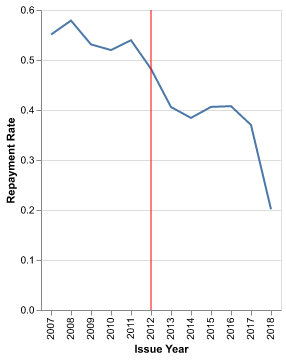
\includegraphics[width=2.97917in,height=3.75in]{pset2_template_files/figure-pdf/cell-21-output-1.png}

While the repayment rate was already on downward trajectory, with the
introduction of the new policy in 2012 the repayment rate continued to
delcine from approximately 52\% in 2011 all the way down to
approximately 20\% in 2018.

\begin{enumerate}
\def\labelenumi{\arabic{enumi}.}
\setcounter{enumi}{5}
\tightlist
\item
\end{enumerate}

\begin{Shaded}
\begin{Highlighting}[]
\CommentTok{\#\#subset data to just pre{-}policy implemenation yeat}
\NormalTok{df\_before\_2012 }\OperatorTok{=}\NormalTok{ df[df[}\StringTok{\textquotesingle{}issue\_date\textquotesingle{}}\NormalTok{].dt.year }\OperatorTok{\textless{}} \DecValTok{2012}\NormalTok{]}
\end{Highlighting}
\end{Shaded}

\begin{Shaded}
\begin{Highlighting}[]
\CommentTok{\#\#find the violation codes that are issued most often}
\NormalTok{df\_before\_2012[}\StringTok{\textquotesingle{}violation\_code\textquotesingle{}}\NormalTok{].value\_counts().head(}\DecValTok{10}\NormalTok{)}
\end{Highlighting}
\end{Shaded}

\begin{verbatim}
violation_code
0976160F    21906
0964190     18117
0964040B    14740
0964090E    11452
1111111     10558
0964150B     9673
0976160A     8339
0964080A     7121
0964190A     3503
0964080B     3435
Name: count, dtype: int64
\end{verbatim}

\begin{Shaded}
\begin{Highlighting}[]
\CommentTok{\#\#create a new column to calculate repayment rate}
\NormalTok{df\_before\_2012[}\StringTok{\textquotesingle{}paid\textquotesingle{}}\NormalTok{] }\OperatorTok{=}\NormalTok{ df[}\StringTok{\textquotesingle{}ticket\_queue\textquotesingle{}}\NormalTok{].}\BuiltInTok{apply}\NormalTok{(}\KeywordTok{lambda}\NormalTok{ x: }\DecValTok{1} \ControlFlowTok{if}\NormalTok{ x }\OperatorTok{==} \StringTok{\textquotesingle{}Paid\textquotesingle{}} \ControlFlowTok{else} \DecValTok{0}\NormalTok{)}
\end{Highlighting}
\end{Shaded}

\begin{Shaded}
\begin{Highlighting}[]
\CommentTok{\#\#calculating repayment rate for violation code 0976160F}
\NormalTok{rate\_1\_test }\OperatorTok{=}\NormalTok{ df\_before\_2012[df\_before\_2012[}\StringTok{\textquotesingle{}violation\_code\textquotesingle{}}\NormalTok{] }\OperatorTok{==} \StringTok{\textquotesingle{}0976160F\textquotesingle{}}\NormalTok{]}
\BuiltInTok{print}\NormalTok{(rate\_1\_test[}\StringTok{\textquotesingle{}paid\textquotesingle{}}\NormalTok{].mean())}
\end{Highlighting}
\end{Shaded}

\begin{verbatim}
0.6078699899570894
\end{verbatim}

\begin{Shaded}
\begin{Highlighting}[]
\CommentTok{\#\#calculating total number of paid tickets for violation code 0976160F}
\NormalTok{rate\_1\_test[}\StringTok{\textquotesingle{}paid\textquotesingle{}}\NormalTok{].}\BuiltInTok{sum}\NormalTok{()}
\end{Highlighting}
\end{Shaded}

\begin{verbatim}
np.int64(13316)
\end{verbatim}

Number of tickets given for violation code 0976160F: 21906 Repayment
rate for violation code 0976160F: 61\% Number of tickets paid: 13316

\begin{Shaded}
\begin{Highlighting}[]
\NormalTok{rate\_2\_test }\OperatorTok{=}\NormalTok{ df\_before\_2012[df\_before\_2012[}\StringTok{\textquotesingle{}violation\_code\textquotesingle{}}\NormalTok{] }\OperatorTok{==} \StringTok{\textquotesingle{}0964190\textquotesingle{}}\NormalTok{]}
\BuiltInTok{print}\NormalTok{(rate\_2\_test[}\StringTok{\textquotesingle{}paid\textquotesingle{}}\NormalTok{].mean())}
\end{Highlighting}
\end{Shaded}

\begin{verbatim}
0.8047690014903129
\end{verbatim}

\begin{Shaded}
\begin{Highlighting}[]
\NormalTok{rate\_2\_test[}\StringTok{\textquotesingle{}paid\textquotesingle{}}\NormalTok{].}\BuiltInTok{sum}\NormalTok{()}
\end{Highlighting}
\end{Shaded}

\begin{verbatim}
np.int64(14580)
\end{verbatim}

Number of tickets given for violation code 0964190: 18117 Repayment rate
for violation code 0976160F: 80\% Number of tickets paid: 14580

\begin{Shaded}
\begin{Highlighting}[]
\CommentTok{\#\#filter the df to only contain the top 10 most frequently given tickets}
\NormalTok{top\_10\_tickets }\OperatorTok{=}\NormalTok{ [}\StringTok{\textquotesingle{}0976160F\textquotesingle{}}\NormalTok{, }\StringTok{\textquotesingle{}0964190\textquotesingle{}}\NormalTok{, }\StringTok{\textquotesingle{}0964040B\textquotesingle{}}\NormalTok{, }\StringTok{\textquotesingle{}0964090E\textquotesingle{}}\NormalTok{, }\StringTok{\textquotesingle{}1111111\textquotesingle{}}\NormalTok{, }\StringTok{\textquotesingle{}0964150B\textquotesingle{}}\NormalTok{, }\StringTok{\textquotesingle{}0976160A\textquotesingle{}}\NormalTok{, }\StringTok{\textquotesingle{}0964080A\textquotesingle{}}\NormalTok{, }\StringTok{\textquotesingle{}0964190A\textquotesingle{}}\NormalTok{, }\StringTok{\textquotesingle{}0964080B\textquotesingle{}}\NormalTok{]}

\NormalTok{most\_frequent\_tickets\_df }\OperatorTok{=}\NormalTok{ df\_before\_2012[df\_before\_2012[}\StringTok{\textquotesingle{}violation\_code\textquotesingle{}}\NormalTok{].isin(top\_10\_tickets)]}

\CommentTok{\#\#group by \textquotesingle{}violation\_code\textquotesingle{} and sum the \textquotesingle{}paid\textquotesingle{} column to get the total count of paid tickets}
\NormalTok{grouped\_by\_code\_df }\OperatorTok{=}\NormalTok{ most\_frequent\_tickets\_df.groupby(}\StringTok{\textquotesingle{}violation\_code\textquotesingle{}}\NormalTok{, as\_index}\OperatorTok{=}\VariableTok{False}\NormalTok{)[}\StringTok{\textquotesingle{}paid\textquotesingle{}}\NormalTok{].}\BuiltInTok{sum}\NormalTok{()}
\end{Highlighting}
\end{Shaded}

\begin{Shaded}
\begin{Highlighting}[]
\CommentTok{\#\#Create the bar chart in Altair}
\NormalTok{q\_2\_6\_chart }\OperatorTok{=}\NormalTok{ alt.Chart(grouped\_by\_code\_df).mark\_bar().encode(}
\NormalTok{    x}\OperatorTok{=}\NormalTok{alt.X(}\StringTok{\textquotesingle{}violation\_code:N\textquotesingle{}}\NormalTok{, title}\OperatorTok{=}\StringTok{\textquotesingle{}Violation Code\textquotesingle{}}\NormalTok{),}
\NormalTok{    y}\OperatorTok{=}\NormalTok{alt.Y(}\StringTok{\textquotesingle{}paid:Q\textquotesingle{}}\NormalTok{, title}\OperatorTok{=}\StringTok{\textquotesingle{}Total Paid Tickets\textquotesingle{}}\NormalTok{),}
\NormalTok{    tooltip}\OperatorTok{=}\NormalTok{[}\StringTok{\textquotesingle{}violation\_code\textquotesingle{}}\NormalTok{, }\StringTok{\textquotesingle{}paid\textquotesingle{}}\NormalTok{]}
\NormalTok{).properties(}
\NormalTok{    title}\OperatorTok{=}\StringTok{"Total Paid Tickets for Each Violation Code"}
\NormalTok{)}
\NormalTok{q\_2\_6\_chart}
\end{Highlighting}
\end{Shaded}

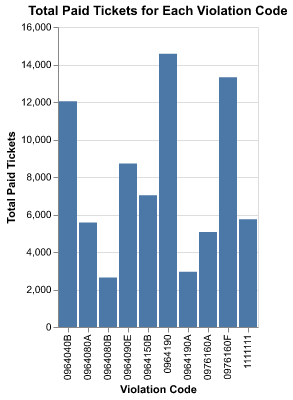
\includegraphics[width=3.05208in,height=4.16667in]{pset2_template_files/figure-pdf/cell-30-output-1.png}

Based on the number of paid tickets by violation types before 2012, if
the city raised the price for each ticket by the same amount (say by
\$80 as it was raised for the no city sticker violation) and wanted to
raise the highest number of revenue, by looking at this chart we can see
that they should increase the price of violation codes 0964190,
0976160F, and 0964040B.

\subsection{Headlines and sub-messages (20
points)}\label{headlines-and-sub-messages-20-points}

\begin{enumerate}
\def\labelenumi{\arabic{enumi}.}
\tightlist
\item
\item
\item
\end{enumerate}

\subsection{Understanding the structure of the data and summarizing it
(Lecture 5, 20
Points)}\label{understanding-the-structure-of-the-data-and-summarizing-it-lecture-5-20-points}

\begin{enumerate}
\def\labelenumi{\arabic{enumi}.}
\tightlist
\item
\item
\item
\end{enumerate}

\subsection{Multi-view Composition (15
Points)}\label{multi-view-composition-15-points}

\begin{enumerate}
\def\labelenumi{\arabic{enumi}.}
\tightlist
\item
\item
\end{enumerate}

\subsection{Extra Credit (max 5
points)}\label{extra-credit-max-5-points}

\begin{enumerate}
\def\labelenumi{\arabic{enumi}.}
\tightlist
\item
\item
\end{enumerate}




\end{document}
